\documentclass[tikz]{standalone}
\usepackage{tikz}

\begin{document}
    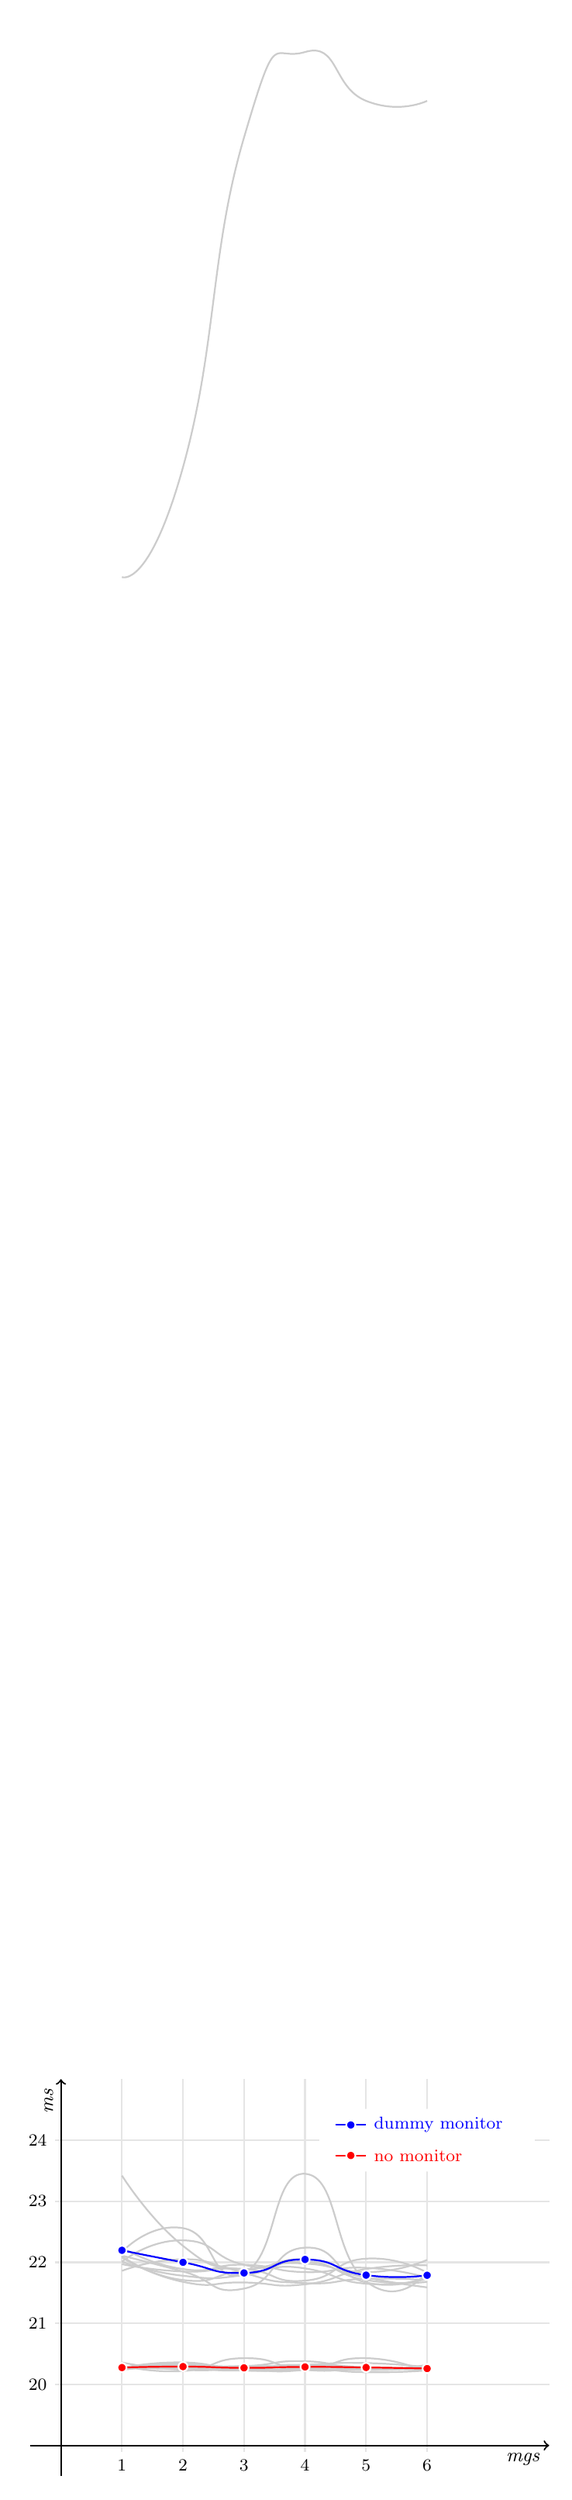
\begin{tikzpicture}[thick]

        \draw[gray!20] (-0.1, 20) node[left, black]{\footnotesize 20} -- (8, 20);
        \draw[gray!20] (-0.1, 21) node[left, black]{\footnotesize 21} -- (8, 21);
        \draw[gray!20] (-0.1, 22) node[left, black]{\footnotesize 22} -- (8, 22);
        \draw[gray!20] (-0.1, 23) node[left, black]{\footnotesize 23} -- (8, 23);
        \draw[gray!20] (-0.1, 24) node[left, black]{\footnotesize 24} -- (8, 24);

        \draw[gray!20] (1, 18.9) node[below, black]{\footnotesize 1} -- (1, 25);
        \draw[gray!20] (2, 18.9) node[below, black]{\footnotesize 2} -- (2, 25);
        \draw[gray!20] (3, 18.9) node[below, black]{\footnotesize 3} -- (3, 25);
        \draw[gray!20] (4, 18.9) node[below, black]{\footnotesize 4} -- (4, 25);
        \draw[gray!20] (5, 18.9) node[below, black]{\footnotesize 5} -- (5, 25);
        \draw[gray!20] (6, 18.9) node[below, black]{\footnotesize 6} -- (6, 25);

        \draw[->] (0, 18.5) -- (0, 25) node[above left, rotate=90]{\small \textit{ms}};
        \draw[->] (-0.5, 19) -- (8, 19) node[below left]{\small \textit{mgs}};


        \draw[gray!40] plot [smooth, tension=1] coordinates {(1, 20.24) (2, 20.31) (3, 20.3) (4, 20.38) (5, 20.24) (6, 20.3)};
        \draw[gray!40] plot [smooth, tension=1] coordinates {(1, 20.26) (2, 20.32) (3, 20.25) (4, 20.32) (5, 20.35) (6, 20.28)};
        \draw[gray!40] plot [smooth, tension=1] coordinates {(1, 20.25) (2, 20.29) (3, 20.24) (4, 20.24) (5, 20.43) (6, 20.2)};
        \draw[gray!40] plot [smooth, tension=1] coordinates {(1, 20.28) (2, 20.26) (3, 20.3) (4, 20.29) (5, 20.26) (6, 20.28)};
        \draw[gray!40] plot [smooth, tension=1] coordinates {(1, 20.27) (2, 20.36) (3, 20.23) (4, 20.26) (5, 20.2) (6, 20.23)};
        \draw[gray!40] plot [smooth, tension=1] coordinates {(1, 20.24) (2, 20.31) (3, 20.23) (4, 20.24) (5, 20.24) (6, 20.26)};
        \draw[gray!40] plot [smooth, tension=1] coordinates {(1, 20.29) (2, 20.27) (3, 20.23) (4, 20.32) (5, 20.28) (6, 20.24)};
        \draw[gray!40] plot [smooth, tension=1] coordinates {(1, 20.31) (2, 20.22) (3, 20.43) (4, 20.24) (5, 20.26) (6, 20.24)};
        \draw[gray!40] plot [smooth, tension=1] coordinates {(1, 20.36) (2, 20.24) (3, 20.27) (4, 20.32) (5, 20.24) (6, 20.32)};
        \draw[gray!40] plot [smooth, tension=1] coordinates {(1, 20.26) (2, 20.34) (3, 20.24) (4, 20.26) (5, 20.28) (6, 20.25)};

        \draw[gray!40] plot [smooth, tension=1] coordinates {(1, 22.24) (2, 21.89) (3, 21.96) (4, 21.84) (5, 21.91) (6, 21.75)};
        \draw[gray!40] plot [smooth, tension=1] coordinates {(1, 22.17) (2, 22.56) (3, 21.83) (4, 23.45) (5, 21.69) (6, 21.84)};
        \draw[gray!40] plot [smooth, tension=1] coordinates {(1, 22.08) (2, 21.68) (3, 21.67) (4, 21.64) (5, 21.89) (6, 21.95)};
        \draw[gray!40] plot [smooth, tension=1] coordinates {(1, 22.11) (2, 21.85) (3, 21.57) (4, 22.24) (5, 21.67) (6, 21.77)};
        \draw[gray!40] plot [smooth, tension=1] coordinates {(1, 22.01) (2, 21.78) (3, 21.79) (4, 22.01) (5, 21.71) (6, 21.68)};
        \draw[gray!40] plot [smooth, tension=1] coordinates {(1, 21.97) (2, 21.85) (3, 21.89) (4, 21.7) (5, 22.06) (6, 21.83)};
        \draw[gray!40] plot [smooth, tension=1] coordinates {(1, 22.1) (2, 21.71) (3, 21.87) (4, 21.98) (5, 21.75) (6, 21.59)};
        \draw[gray!40] plot [smooth, tension=1] coordinates {(1, 23.42) (2, 22.27) (3, 21.83) (4, 21.66) (5, 21.73) (6, 21.71)};
        \draw[gray!40] plot [smooth, tension=1] coordinates {(1, 22.01) (2, 22.36) (3, 21.96) (4, 21.9) (5, 21.65) (6, 21.73)};
        \draw[gray!40] plot [smooth, tension=1] coordinates {(1, 21.86) (2, 22.05) (3, 21.89) (4, 22.05) (5, 21.84) (6, 22.04)};


        \draw[red] plot [smooth, tension=1] coordinates { (1, 20.276) (2, 20.292) (3, 20.272) (4, 20.287) (5, 20.278) (6, 20.26)};
        \draw[blue] plot [smooth, tension=1] coordinates { (1, 22.197) (2, 22.0) (3, 21.826) (4, 22.047) (5, 21.79) (6, 21.788)};


        \draw[white, fill=red] (1, 20.276) circle (0.075cm);
        \draw[white, fill=red] (2, 20.292) circle (0.075cm);
        \draw[white, fill=red] (3, 20.272) circle (0.075cm);
        \draw[white, fill=red] (4, 20.287) circle (0.075cm);
        \draw[white, fill=red] (5, 20.278) circle (0.075cm);
        \draw[white, fill=red] (6, 20.26) circle (0.075cm);

        \draw[white, fill=blue] (1, 22.197) circle (0.075cm);
        \draw[white, fill=blue] (2, 22.0) circle (0.075cm);
        \draw[white, fill=blue] (3, 21.826) circle (0.075cm);
        \draw[white, fill=blue] (4, 22.047) circle (0.075cm);
        \draw[white, fill=blue] (5, 21.79) circle (0.075cm);
        \draw[white, fill=blue] (6, 21.788) circle (0.075cm);

        \coordinate (legend) at (4.25, 23.5);
        \draw[white, fill=white, rounded corners] (legend) rectangle ++ (3.5, 1);

        \draw[red] ([shift={(0.25, 0.25)}]legend) -- ++ (0.5, 0) node[right]{\footnotesize no monitor};
        \draw[white, fill=red] ([shift={(0.5, 0.25)}]legend) circle (0.075cm);

        \draw[blue] ([shift={(0.25, 0.75)}]legend) -- ++ (0.5, 0) node[right]{\footnotesize dummy monitor};
        \draw[white, fill=blue] ([shift={(0.5, 0.75)}]legend) circle (0.075cm);

        \draw[gray!40] plot [smooth, tension=1] coordinates { (1, 49.6) (2, 51.4) (3, 56.8) (4, 58.2) (5, 57.4) (6, 57.4) };
    \end{tikzpicture}
\end{document}